
\chapter{Intelligent transportations and Vehicle to everything protocol Examples of IoT, IoT security Artificial Intelligence of Things (AIoT), HW/SW environments for IoT/AIoT}


\chapter{Data Gathering, Data Preprocessing, Data Harmonization for intelligent system learning}

\section{Value of Data Analytic}
\begin{figure}[H]
    \centering
    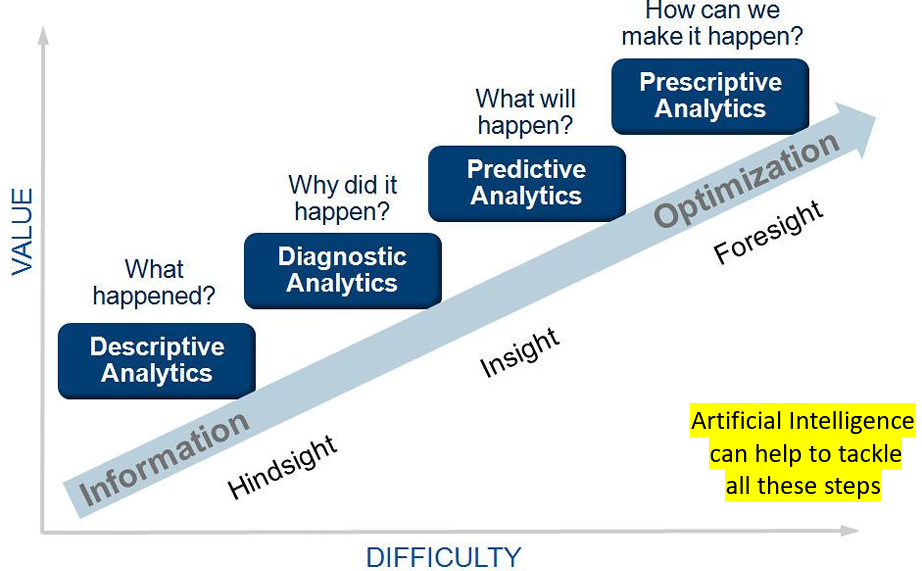
\includegraphics[width=0.8\linewidth]{07-08/images/Data.png}
\end{figure}

Four possibility increasing the value and the difficulty:
\begin{itemize}
    \item Descriptive Analytics
    \item Diagnostic Analystics
    \item Predictive Analytics
    \item Prespective Analaytics
\end{itemize}

\section{Data gathering - Step 1}
\begin{figure}[H]
    \centering
    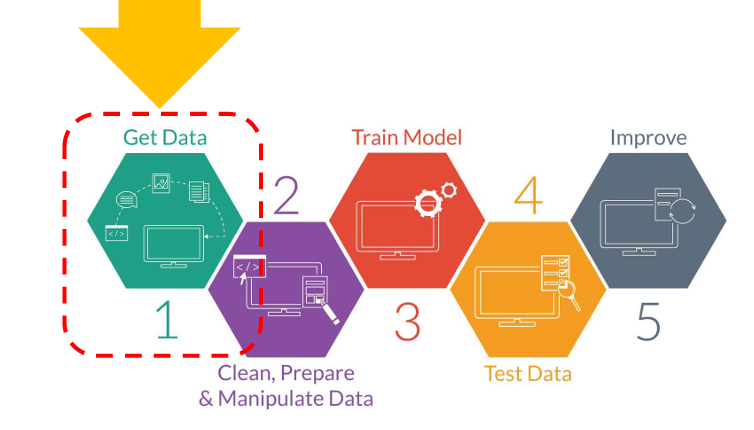
\includegraphics[width=0.8\linewidth]{07-08/images/data ghatering.png}
\end{figure}

\noindent We have so many powerful sources capable to generate data.

\noindent \textbf{Data collection is the process of gathering and measuring information on targeted variables in an established system}

\subsection{IoT started to generate data…}
\noindent The amount of data generated by connected internet of things (IoT) devices, forecast to grow to by 2025
\begin{itemize}
    \item 41.6 billion connected devices
    \item 79.4 zettabytes (ZB) of data/year.
\end{itemize} 

\noindent Data sources like phones, smart watches, ecc..

\begin{figure}[H]
    \centering
    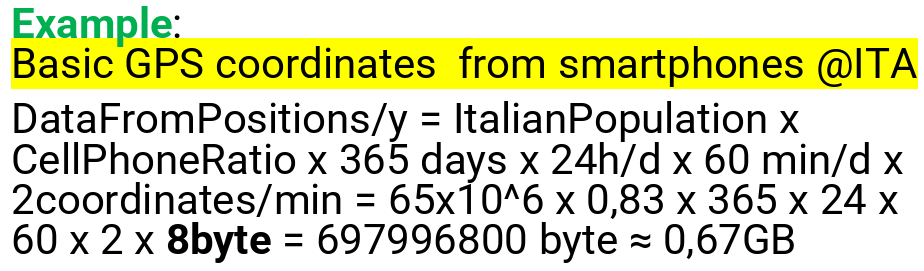
\includegraphics[width=0.8\linewidth]{07-08/images/example 1.png}
\end{figure}

\noindent There are pubblic data centers, like Amazon's, Google's and Governative's ones

\subsection{Data heterogeneity and synchronization}
\noindent  Heterogeneity in statistics means that your populations, samples or results are different. It is the opposite of homogeneity which means that the, population/data/results are the same.
Qua fa un tot di esempi  su come sia importante avere tutti i dati nello stesso formato (esempio di Marte e della NASA e della wind station)

\subsection{Data Synchronization}
\noindent The way a device adjusts its internal clock in order to align with the clocks of other devices in a network

\subsubsection{Network Time Synchronization}
Computer clocks in servers, workstations and network devices are inherently not enough accurate
Two problems:
\begin{itemize}
    \item Clocks are set by hand to within a minute or two of actual time and are rarely checked after that 
    \item Clocks are maintained by a battery-backed device that may drift as much as a second per day 
\end{itemize}
\noindent \textbf{It’s impossible to have accurate time synchronization without a proper method}

\subsubsection{Solutions}
\begin{itemize}
    \item \textbf{Network Time Protocol (NTP):} is a protocol for clock synchronization between computer systems over packetswitched, variable-latency data networks designed to mitigate local network latency 
    \item \textbf{Time Server:} Dedicated network Time Server behind your firewall (devices synchronized to within 1/2 to 2 ms)
\end{itemize}

\begin{figure}[H]
    \centering
    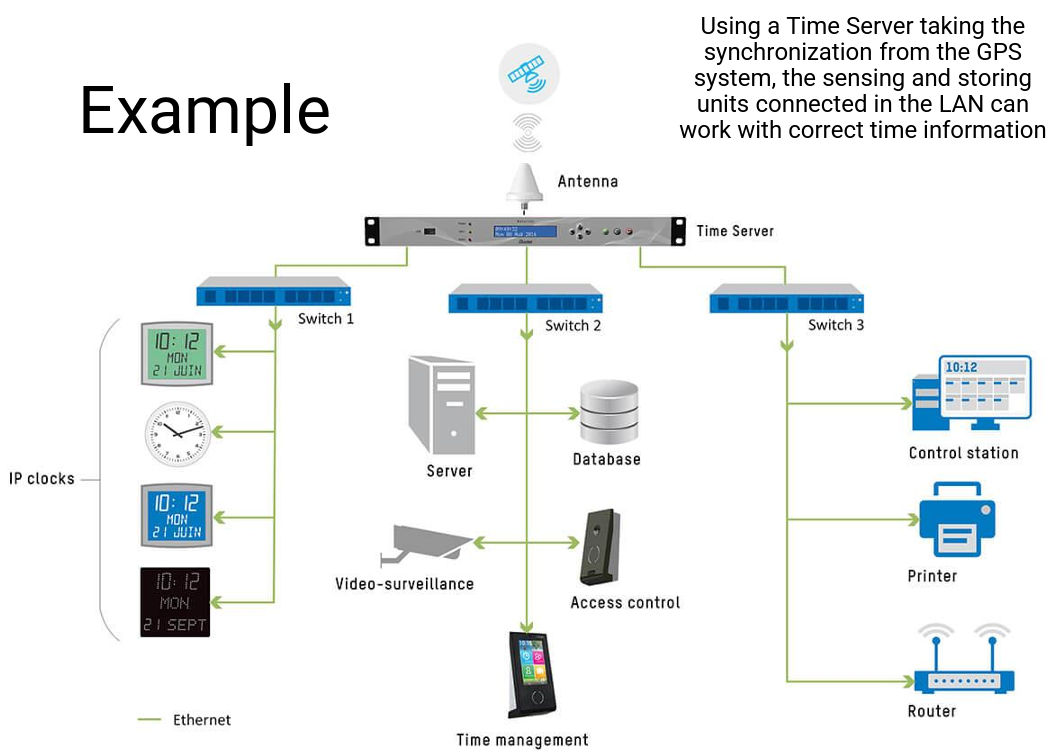
\includegraphics[width=0.8\linewidth]{07-08/images/sync.png}
\end{figure}


\section{Data Preparation - Step 2}
\begin{figure}[H]
    \centering
    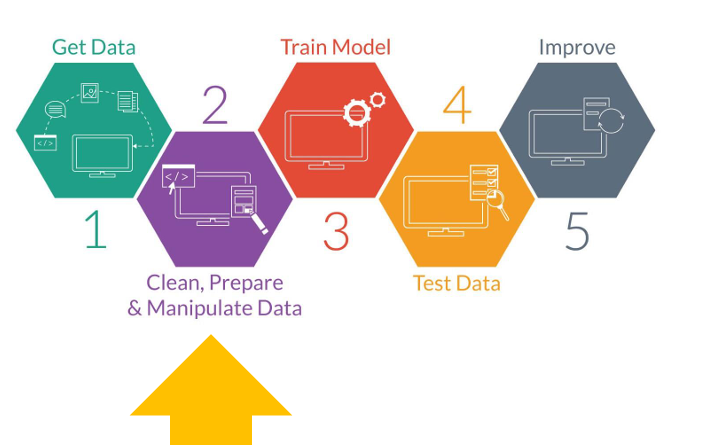
\includegraphics[width=0.8\linewidth]{07-08/images/step2.png}
\end{figure}

\noindent Data preparation includes two concepts such as Data Cleaning and Feature Engineering

\noindent The data wrangling problem is growing as different types of unstructured data or data in varying formats are pouring in from sensors, online and from traditional databases. 
All these data must be \textbf{cleaned up and organized } before data analytics/classifiers/regressors models can be applied.

\subsection{Data wrangling}
\noindent Data wrangling steps:
\begin{itemize}
    \item Iterative process
    \item Understand
    \item Explore
    \item Transform
    \item Augment
    \item Visualize
\end{itemize}

\begin{figure}[H]
    \centering
    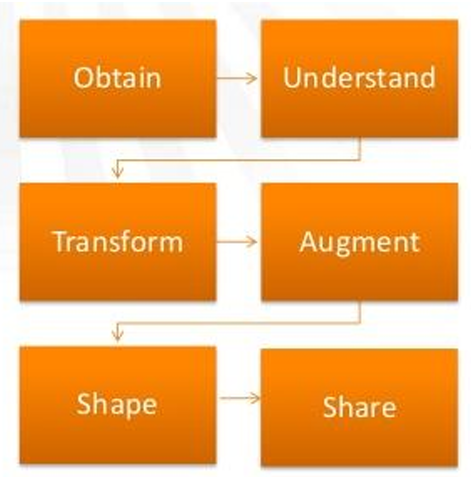
\includegraphics[width=0.6\linewidth]{07-08/images/data wrangling.png}
\end{figure}

\noindent Tasks of Data Wrangling:
\begin{itemize}
    \item \textbf{Discovering:} Firstly, data should be understood thoroughly and examine which approach will best suit. 
    \item \textbf{Structuring:} As the data is gathered from different sources, the data will be present in various shapes and sizes. Therefore, there is a need for structuring the data in proper format.
    \item \textbf{Cleaning:} Cleaning or removing of data should be performed that can degrade the performance of analysis.
    \item \textbf{Enrichment:} Extract new features or data from the given data set to optimize the performance of the applied model.
    \item \textbf{\textit{Validating:}} This approach is used for improving the quality of data and consistency rules so that transformations that are applied to the data could be verified.
\end{itemize}

\noindent \textbf{Data pre-processing:} "is a technique that is used to convert the raw data into a clean data set"
\noindent Pre-processing includes • Data cleaning • Data integration • Data transformation • Data reduction

\noindent \textbf{Why is Data Preprocessing is so important?}
\noindent Three answers:
\begin{itemize}
    \item Inaccurate data (missing data) 
    \item The presence of noisy data/erroneous data/outliers
    \item Inconsistent data 
\end{itemize}

\subsection{Missing Data}
\noindent What do we do when we have missing data? 
\begin{itemize}
    \item \textbf{Ignoring the missing record:} is the simplest and efficient method for handling the missing data (not the best method when the number of missing values are immense or  when the missing data problem and can solved (debugging/re-designredoing the experiment) and not just ignoring the problem causing the missing data.). 
    \item \textbf{Filling the missing values manually:} one of the best-chosen methods, But there is one limitation that when there are large data set, and missing values are significant then, this approach is not efficient as it becomes a timeconsuming task.
    \item \textbf{Filling using computed values:} The missing values can also be occupied by computing mean, mode or median of the observed given values (ex: you can copy from the most similar column or generate values by using any ML or Deep Learning algorithm but  it can generate bias within the data). 
\end{itemize}

\begin{figure}[H]
    \centering
    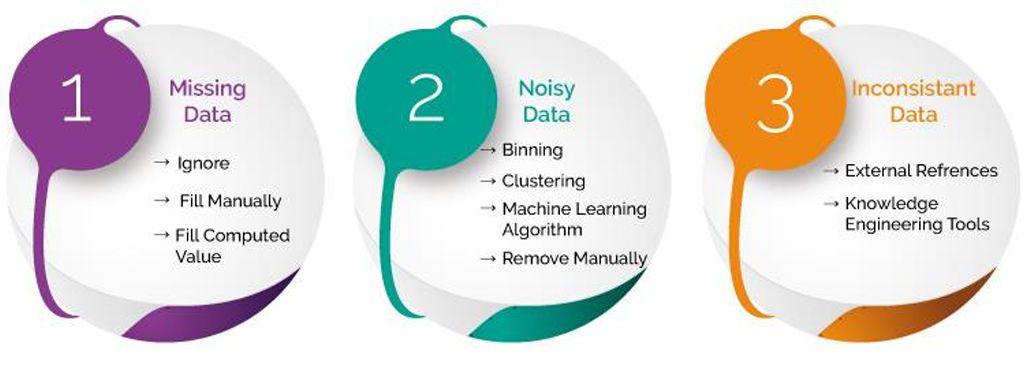
\includegraphics[width=0.8\linewidth]{07-08/images/data missing.png}
\end{figure}

\subsection{Structured and unstructured Data }
\noindent \textbf{Structured data} usually resides in relational databases, This format is eminently searchable both with human generated queries and via algorithms using type of data and field names, such as alphabetical or numeric, currency or date.

\noindent \textbf{Unstructured data} is essentially everything else. Unstructured data has internal structure but is not structured via pre-defined data models or schema (ex: sensor data, text files, emails, etc..).

\subsubsection{Neural networks and unstructured data}
\noindent It is not strictly compulsory to have structured data to use ML 

\begin{figure}[H]
    \centering
    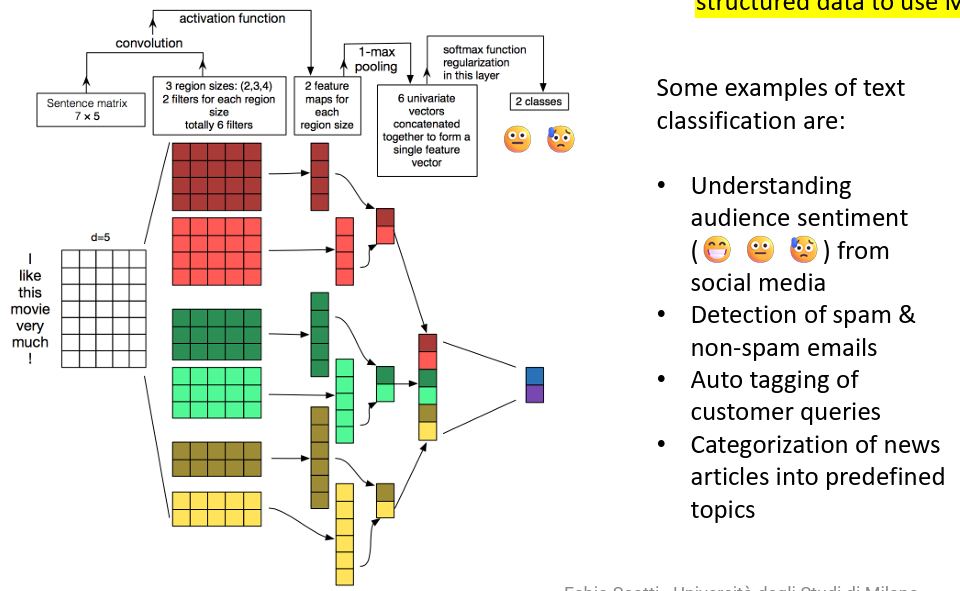
\includegraphics[width=0.8\linewidth]{07-08/images/unstructured data.png}
\end{figure}



\chapter{Managing a small dataset in Python Degrees of freedom/parameters Data Leakage}
Lab in Pythone, c'è codice all'esame ma non che dobbiamo fare noi da zero( però possibili domande sul codice)


\section{Degrees of freedom /parameters of the models - Step 1 and 3}


\begin{figure}[H]
    \centering
    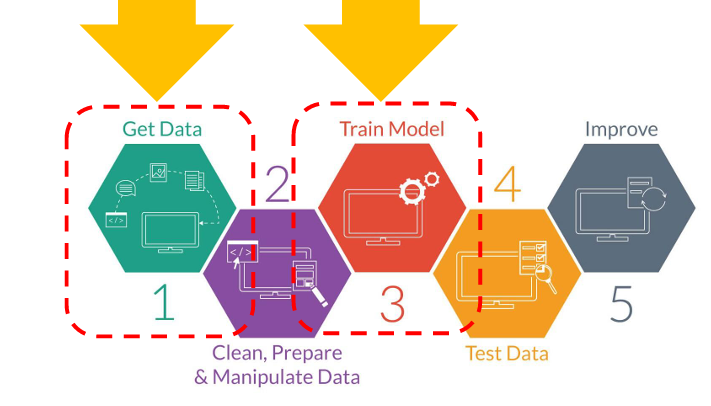
\includegraphics[width=0.8\linewidth]{07-08/images/step 1 and 3.png}
\end{figure}

\subsection{How much data? Degree of freedom/parameters}
\noindent In physics, the degree of freedom of a mechanical system is the number of independent parameters that define its configuration.

\noindent Note: DoF is not exactly equivalent Par for complex systems, but they are strongly related.

\subsection{Similitude 1}
\begin{figure}[H]
    \centering
    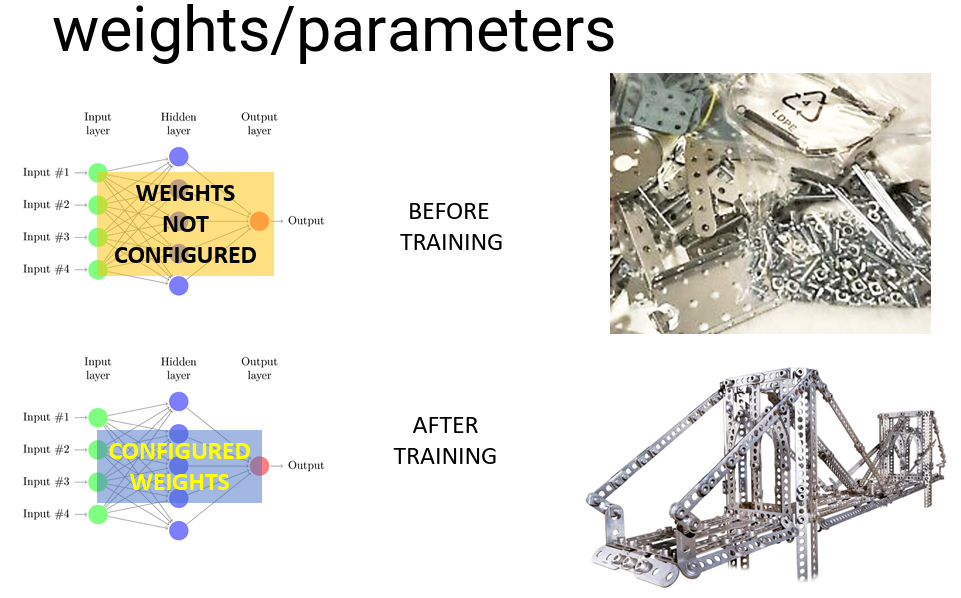
\includegraphics[width=0.8\linewidth]{07-08/images/similitude 1.png}
\end{figure}

\subsection{Similitude 2}
\begin{figure}[H]
    \centering
    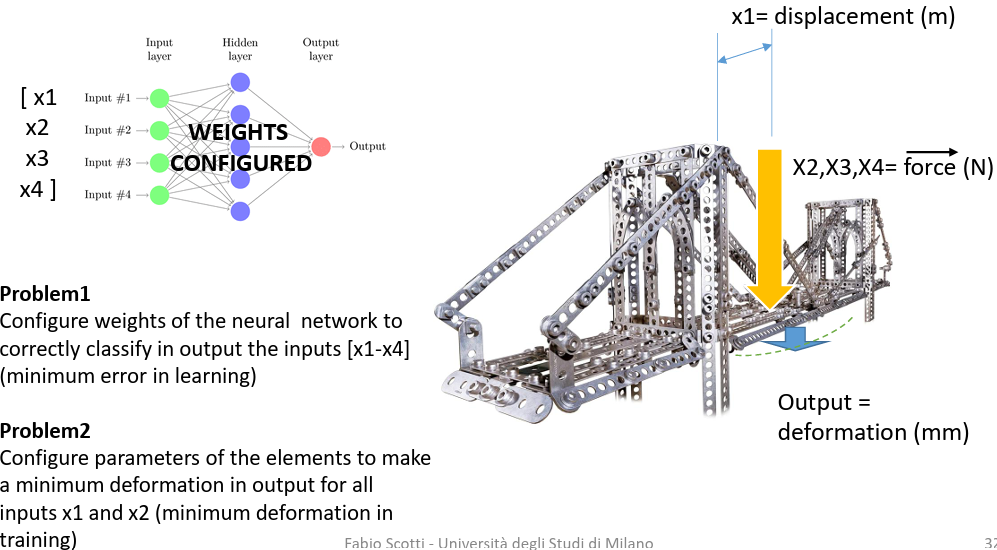
\includegraphics[width=0.8\linewidth]{07-08/images/similitude 2.png}
\end{figure}

\subsection{Number of Parameters of NNs}
\begin{figure}[H]
    \centering
    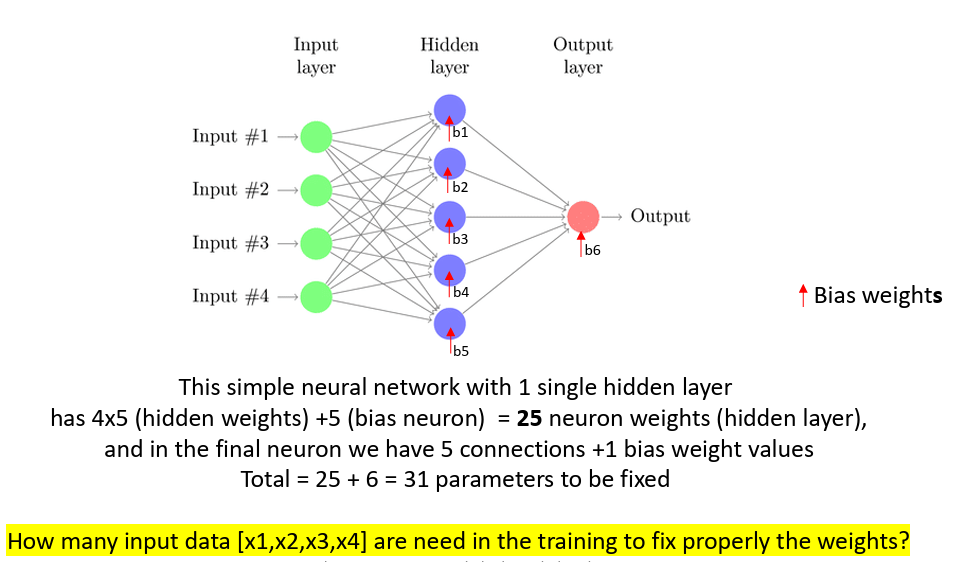
\includegraphics[width=0.8\linewidth]{07-08/images/nns.png}
\end{figure}

\subsection{a 1D linear model}
\noindent We have the weight (w1) and the bias (beta)
\begin{figure}[H]
    \centering
    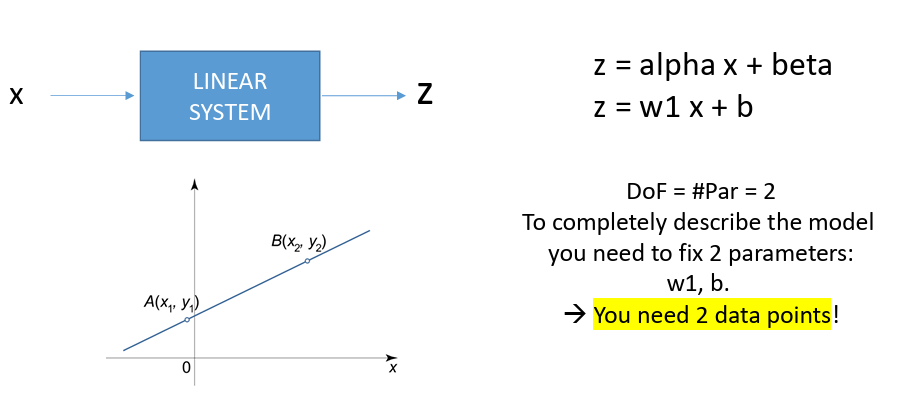
\includegraphics[width=0.8\linewidth]{07-08/images/d1.png}
\end{figure}

\subsection{a 2D linear model}
Now we have 3 parameters to fix
\begin{figure}[H]
    \centering
    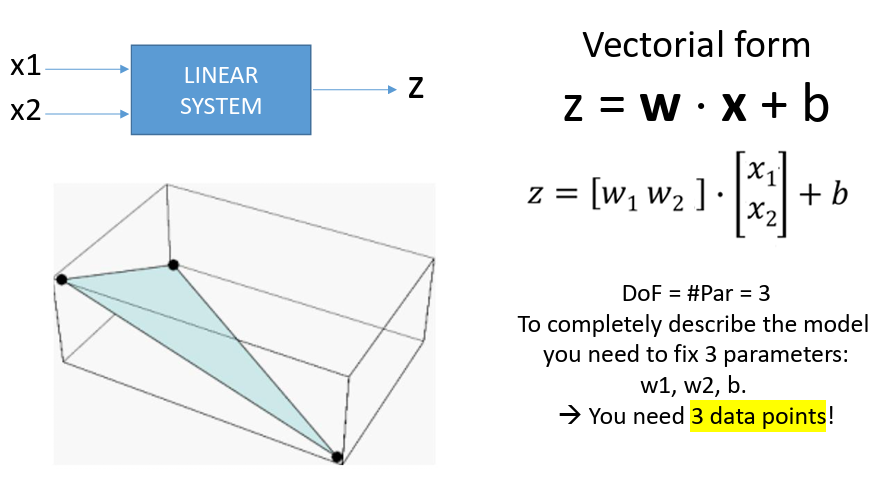
\includegraphics[width=0.8\linewidth]{07-08/images/2d.png}
\end{figure}

\subsection{a 3D linear model}
Increasing the number of inputs I increas the number of parameters to fix
\begin{figure}[H]
    \centering
    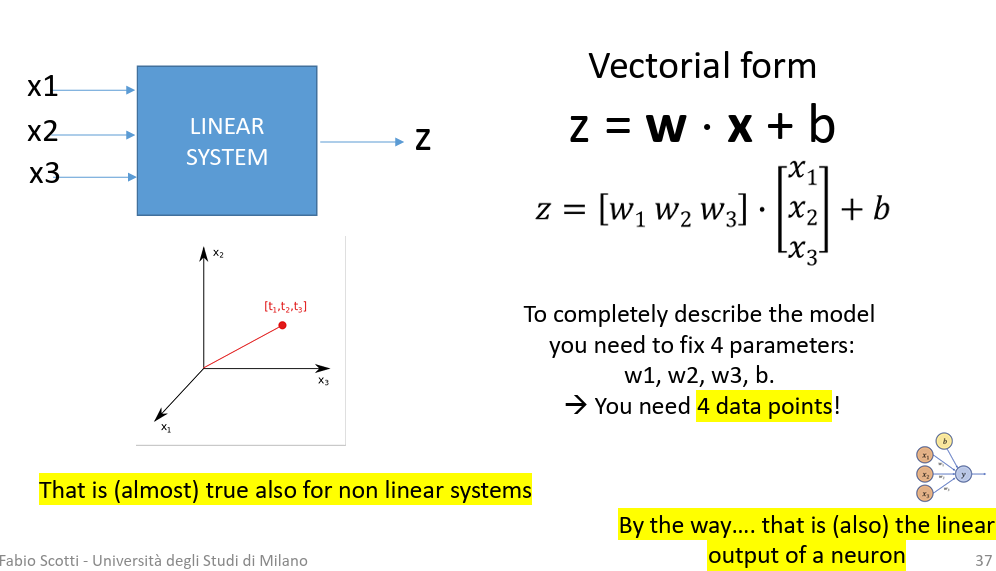
\includegraphics[width=0.8\linewidth]{07-08/images/3d.png}
\end{figure}

\subsection{DoF in general}
\noindent The degrees of freedom for a given problem are the number of independent problem variables which must be specified to uniquely determine a solution.

\begin{itemize}
    \item degrees of freedom = variables - equations
    \item database are vectors so number of data = number of vectors in our database
\end{itemize}

\subsection{In brief...}
\begin{itemize}
    \item The number of Par of the model (e.g., neural network) must be carfully tuned according to
    \begin{itemize}
        \item the size of the datasets (Number of vectors, Number of inputs)
        \item its complexity 
    \end{itemize}
\end{itemize}

\noindent \textbf{\textit{«Go deep» only if it is really necessary }}


\section{Data leakage - Step 2}
\noindent Data Leakage is responsible for the cause of invalid Machine Learning/Deep Learning model due to the over optimization of the applied model.
\begin{figure}[H]
    \centering
    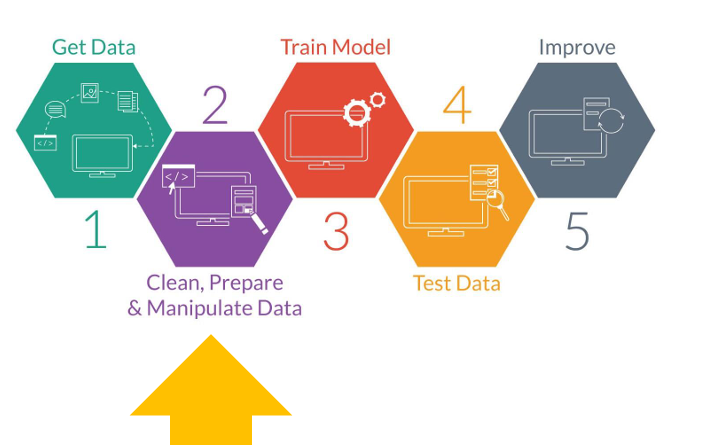
\includegraphics[width=0.8\linewidth]{07-08/images/step2.png}
\end{figure}

\noindent Two main topics:
\begin{itemize}
    \item \textbf{Missing relevant features: }For example, when we want to use a particular feature for performing Predictive Analysis, but that specific feature is 
    not present at the time of training of dataset (Example: you want to add to your dataset the concentration of OrmonX to predict CancerZ but OrmonX is not (almost) present in the trainig dataset.)
    \begin{figure}[H]
        \centering
        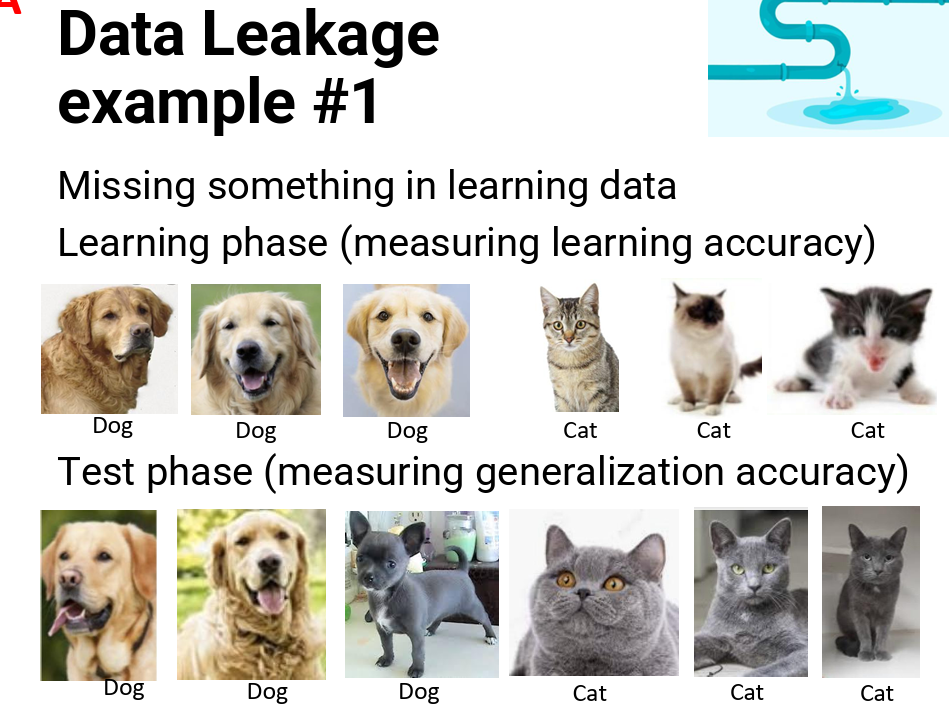
\includegraphics[width=0.8\linewidth]{07-08/images/cani e gatti.png}
    \end{figure}
    \item \textbf{Adding something more..:}When information from outside the “expected” training information in the dataset is used to create the model. This additional information can allow the model to learn or know something that it otherwise would not know and in turn invalidate the estimated performance of the model being constructed.
    This additional learning of information by the applied model will disapprove the computed estimated generalization performance of the model, your performance estimation of the model once it will be deployed tends to be too much optimistic.
\end{itemize}
\begin{figure}[H]
    \centering
    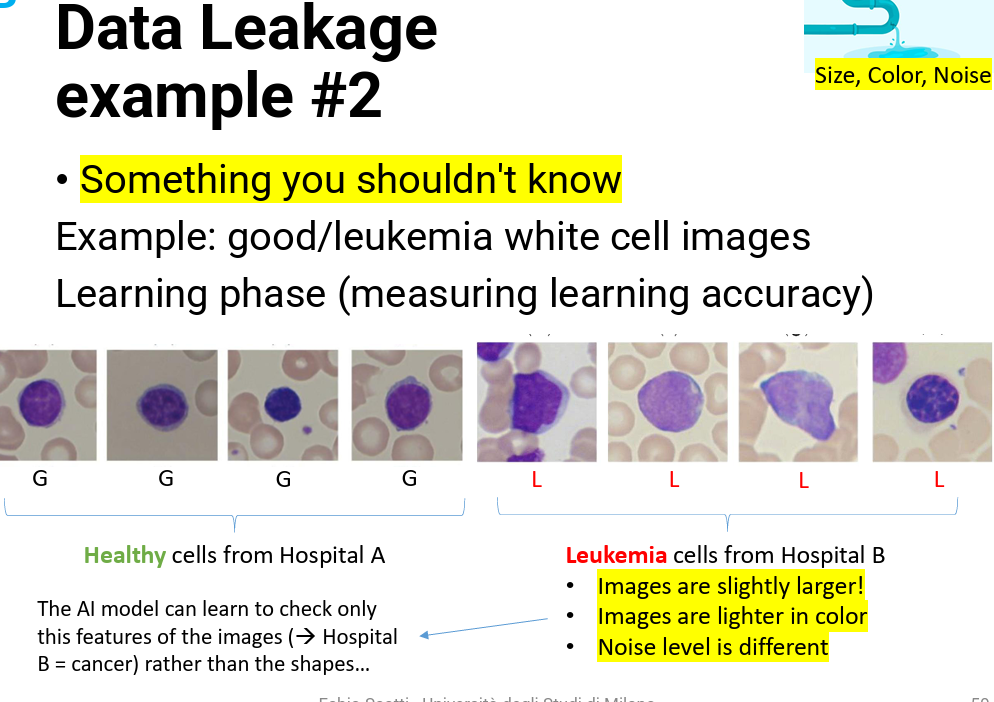
\includegraphics[width=0.8\linewidth]{07-08/images/leucemia.png}
\end{figure}

\subsection{Data Leakage can happen}
\begin{itemize}
    \item The Leakage of data from test dataset to training dataset
    \item Leakage of future data into the past data
    \item  Usage of data outside the scope of the applied algorithm
\end{itemize}


\noindent In brief, we have two primary sources of data leakage in Machine Learning algorithms:
\begin{itemize}
    \item \textbf{Feature attributes (variables are saying too much…) }
    \item \textbf{Training data set (chunk of data used in the wrong phase) }
\end{itemize}

\subsection{Time series: a special case for Regression and Classification}
\begin{figure}[H]
    \centering
    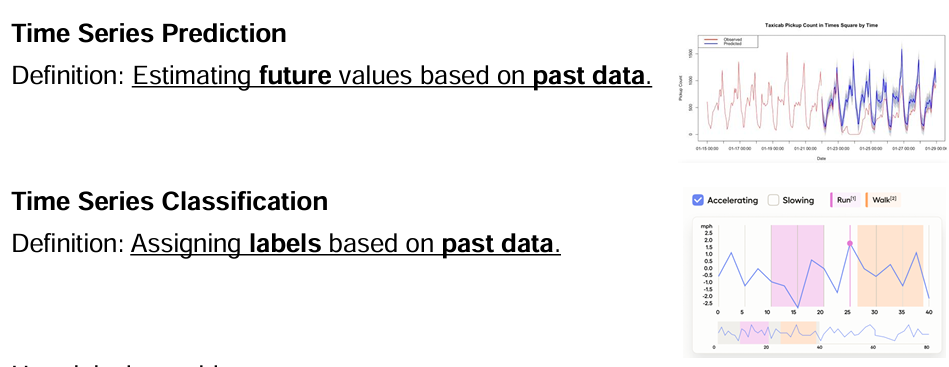
\includegraphics[width=0.8\linewidth]{07-08/images/time series.png}
\end{figure}

\noindent \textbf{Problem:} in both cases, the model can be effective is the past data is consistent 
\begin{itemize}
    \item \textit{training} (input to the learning method)
    \item \textit{inference}(input to the model)
\end{itemize}

\noindent Data Leakage is observed in time-related complex datasets such as: 
dividing time series the dataset can be an error-prone problem

\subsection{Checking the presence of Data Leakage}
Data Leakage is observed in timerelated complex datasets such as: 
\begin{itemize}
    \item Storage of analog observations in the form of audios and images in separate files having a defined size and timestamp
    \item Implementation of sampling in a graphical problem is a complex task
\end{itemize}


\subsubsection{The cropping problem}
\noindent The \textbf{cropping problem} is a form of data leakage that affects multiple types of datasets and applications. It occurs when a model learns patterns from cropped or contextually biased data, leading to misleadingly high performance but poor generalization.

\noindent Is a form of data leakage where you cat to much or not enought information.

\begin{itemize}
    \item \textbf{Images:} A model trained to classify objects may unintentionally rely on cropped edges or artifacts from image preprocessing rather than actual object features.
    \item \textbf{Audio: } A speech recognition model may learn background noise patterns from cropped samples instead of focusing on spoken words.
    \item \textbf{Structured Data:} In medical diagnosis, if training data is cropped to contain only extreme cases, the model might fail on intermediate cases.
    \item \textbf{Unstructured Data (Text):}  A sentiment analysis model trained on social media posts might learn to rely on specific truncated phrases instead of full context.
\end{itemize}

